% !TeX root = ../wireless_networks.tex
\chapter{Wireless LAN}
Some advantages of WLAN are:

\begin{itemize}
\item \textbf{Flexibility}: Within radio coverage, nodes can communicate without further
restriction. Radio waves can penetrate walls, senders and receivers can be
placed anywhere (also non-visible, e.\ g.\ , within devices, in walls etc.).


\item \textbf{Planning}: Only wireless ad-hoc networks allow for communication without previous planning, any wired network needs wiring plans. As long as devices follow the same standard, they can communicate. 

\item \textbf{Design}: Wireless networks allow for the design of small, independent devices which can for example be put into a pocket. Wireless senders and receivers can be hidden in historic buildings,  e.\ g.\ , current networking technology can be introduced without being visible.


\item \textbf{Robustness}: Wireless networks can survive disasters, e.\ g.\ , earthquakes or users pulling a plug. If the wireless devices survive, people can still communicate. 

\item \textbf{Cost}: After providing wireless access to the infrastructure via an access point for the first user, adding additional users to a wireless network will not
increase the cost. This is, important for  e.\ g.\ , lecture halls, hotel lobbies or gate areas in airports where the numbers using the network may vary significantly. 
\end{itemize}


\section{Infrared Vs Radio Transmission}
Two different basic transmission technologies can be used to set up WLANs. One technology is based on the transmission of \textit{infrared light} ( e.\ g.\ , at 900 nm
wavelength), the other one, which is much more popular, uses \textit{radio transmission} in the GHz range ( e.\ g.\ , 2.4 GHz in the license-free ISM band). Both technologies
can be used to set up ad-hoc connections for work groups, to connect,  e.\ g.\ , a desktop with a printer without a wire, or to support mobility within a small area.


\subsection{Infrared Transmission}
\begin{itemize}
	\item Infrared technology uses diffuse light reflected at walls, furniture etc.\ or directed light if a line-of-sight (LOS) exists between sender and receiver. 
	\item Senders can be simple light emitting diodes (LEDs) or laser diodes. 
	\item Photodiodes act as receivers.
\end{itemize}

\begin{multicols}{2}
	\subsubsection*{Advantages}
	\begin{itemize}
		\item The main advantages of infrared technology are its simple and extremely cheap senders and receivers which are integrated into nearly all mobile devices available today. For example, PDAs, laptops, notebooks, mobile phones etc.\ have
		an infra-red data association (IrDA) interface. 
		\item No licenses are needed for infrared technology and shielding is very simple. 
		\item Electrical devices do not interfere with infrared transmission.
	\end{itemize}
\end{multicols}




\begin{multicols}{2}
	\subsubsection*{Disadvantages}
	\begin{itemize}
		\item Disadvantages of infrared transmission are its low bandwidth compared to	other LAN technologies. 
		\item Typically, IrDA devices are internally connected to a serial port limiting transfer rates to 115 kbit/s. 
		\item However, their main disadvantage is that infrared	is quite easily shielded. 
		\item Infrared transmission cannot penetrate walls or other obstacles. 
		\item Typically, for good transmission quality and high data rates a LOS, i.\ e.\, direct connection, is needed.
	\end{itemize}
\end{multicols}

\subsection{Radio Transmission}
HIPERLAN and Bluetooth rely on radio transmission.

\begin{multicols}{2}
\subsubsection*{Advantages}
	\begin{itemize}
		\item Advantages of radio transmission include the long-term experiences made with radio transmission for wide area networks (e.\ g.\ , microwave links) and mobile cellular phones. 
		\item Radio transmission can cover larger areas and can	penetrate (thinner) walls, furniture, plants etc. 
		\item Additional coverage is gained by reflection. 
		\item Radio typically does not need a LOS if the frequencies are not too high. 
		\item Furthermore, current radio-based products offer much	higher transmission rates than infrared.
	\end{itemize}
\end{multicols}



The main advantage is also a big disadvantage of radio transmission.
\begin{multicols}{2}
	\subsubsection*{Disadvantages}
\begin{itemize}
	\item Shielding is not so simple. 
	\item Radio transmission can interfere with other senders, or electrical devices can destroy data transmitted via radio.
	\item Additionally, radio transmission is only permitted in certain frequency bands. 
	\item Very limited ranges of license-free bands are available worldwide and	those that are available are not the same in all countries.
\end{itemize}
\end{multicols}


\section{Infrastructure and Ad-hoc Network}\label{sec:infrastructure-ad-hoc}

\subsection{Infrastructure Network}
Many WLANs of today need an infrastructure network. Infrastructure networks not only provide access to other networks, but also include forwarding functions, medium access control etc. 
\begin{itemize}
	\item In these infrastructure-based wireless networks, communication typically takes place only between the wireless nodes and the access point (see Figure \ref{fig:ad-hoc-network}), but not directly between the wireless nodes.
	\item The access point does not just control medium access, but also acts as a bridge to other wireless or wired networks. Figure \ref{fig:ad-hoc-network} shows three access points with their three wireless networks and a wired network. 
	\item Several wireless networks may form one logical wireless network, so the access points together with the fixed network in between can connect several wireless networks to form a larger network beyond actual radio coverage.
	
\end{itemize}


%--------------------------------------------
%				
%				Figure
%
%--------------------------------------------

\begin{figure}[pht]
\centering
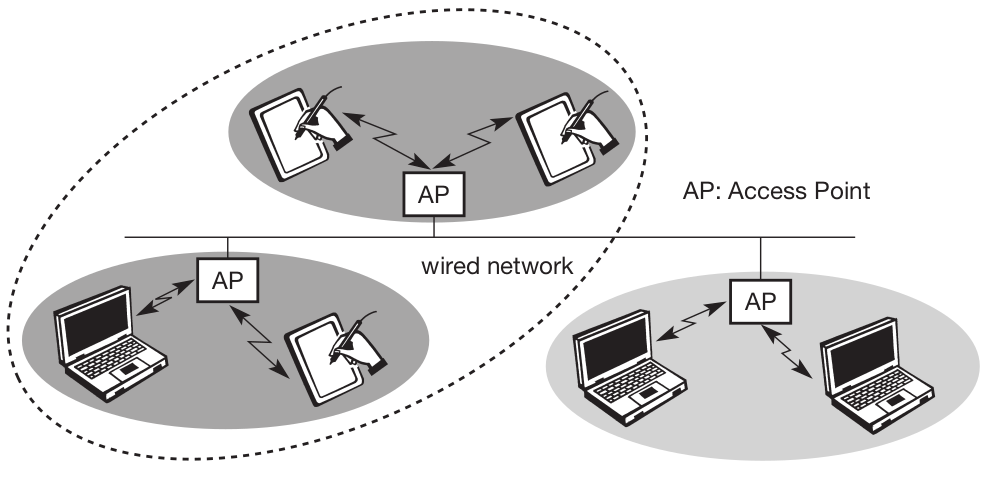
\includegraphics[width=0.8\textwidth]{ad-hoc-network}
\caption{Example of three infrastructure-based wireless networks}\label{fig:ad-hoc-network}
\end{figure}
\subsubsection*{Advantages}
\begin{itemize}
	\item The design of infrastructure-based wireless networks is simpler because most of the network functionality lies within the access point, whereas the wireless clients can remain quite simple. 
	\item If only the access point controls medium access, no collisions are possible. 
	\item This setting may be useful for quality of service guarantees such as minimum bandwidth for certain nodes. 
	\item The access point may poll the single wireless nodes to ensure the data rate.
\end{itemize}

\subsubsection*{Disadvantage(s)}

\begin{itemize}
	\item Infrastructure-based networks lose some of the flexibility wireless networks can offer, e.\ g.\ , they cannot be used for disaster relief in cases where no infrastructure is left. 
\end{itemize}

\noindent Typical cellular phone networks are infrastructure-based networks for a wide area. Also satellite-based cellular phones have an infrastructure - the satellites. Infrastructure does not necessarily imply a wired fixed network.


\subsection{Ad-hoc Network}
\begin{itemize}
	\item Ad-hoc wireless networks, however, do not need any infrastructure to work. 
	\item Each node can communicate directly with other nodes, so no access point controlling medium access is necessary. 
	
\end{itemize}

Figure {\ref{fig:two-ad-hoc-wireless-networks}} shows two ad-hoc networks with three nodes each. Nodes within an ad-hoc network can only communicate if they can reach each other physically, i.\ e.\ , if they are within each other’s radio range or if other nodes can forward the message. Nodes from the two networks shown in Figure {\ref{fig:two-ad-hoc-wireless-networks}} cannot, therefore, communicate with each other if they are not within the same radio range.

%%%%%%%%%%%%%%%%%%%%%%%%%%%%%%%%%%%%%%%%%%%%%%
%				
%				Figure
%
%%%%%%%%%%%%%%%%%%%%%%%%%%%%%%%%%%%%%%%%%%%%%%
\begin{figure}[pht!]
	\centering
	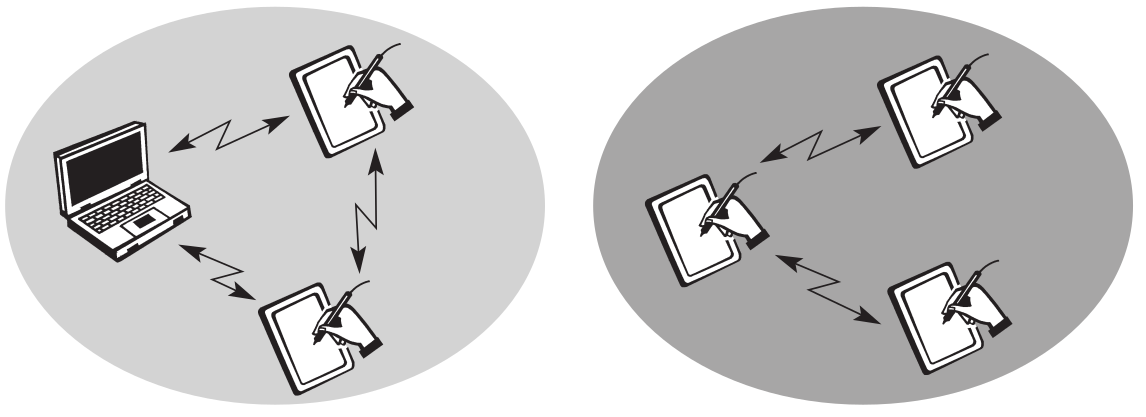
\includegraphics[width=0.8\textwidth]{two-ad-hoc-wireless-networks}
	\caption{Example of two ad-hoc wireless networks}\label{fig:two-ad-hoc-wireless-networks}
\end{figure}

\subsubsection*{Advantage}
\begin{itemize}
	\item This type of wireless network exhibits the greatest possible flexibility as it is, for example, needed for unexpected meetings, quick replacements of infrastructure or communication scenarios far away from any infrastructure.
\end{itemize}
\subsubsection*{Disadvantage}
\begin{itemize}
	\item The complexity of each node is higher because every node has to implement medium access mechanisms, mechanisms to handle hidden or exposed terminal problems, and perhaps priority mechanisms, to provide a certain quality of service.
\end{itemize}




\section{IEEE 802.11}
The IEEE standard 802.11 specifies the most famous family of WLANs in which many products are available. This standard belongs to the group of 802.x LAN standards,  e.\ g.\ , 802.3 Ethernet or 802.5 Token Ring.

The primary goal of the standard was the specification of a simple and robust WLAN which offers time-bounded and asynchronous services. The MAC layer should be able to operate with multiple physical layers, each of which exhibits a different medium sense and transmission characteristic. Candidates for physical layers were infrared and spread spectrum radio transmission techniques.

Additional features of the WLAN should include the support of power management to save battery power, the handling of hidden nodes, and the ability to operate worldwide. The 2.4 GHz ISM band, which is available in most countries around the world, was chosen for the original standard. Data rates envisaged for the standard were 1 Mbit/s mandatory and 2 Mbit/s optional.

\subsection{System Architecture}\label{sec:wireless-network-architecture}
Wireless networks can exhibit two different basic system architectures as shown
in section {\ref{sec:infrastructure-ad-hoc}}: \textit{infrastructure-based} or \textit{ad-hoc}. Figure {\ref{fig:architecture-of-ieee-802-11}} shows the components of an infrastructure and a wireless part as specified for IEEE 802.11. 

%%%%%%%%%%%%%%%%%%%%%%%%%%%%%%%%%%%%%%%%%%%%%%
%				
%				Figure
%
%%%%%%%%%%%%%%%%%%%%%%%%%%%%%%%%%%%%%%%%%%%%%%
\begin{figure}[hpt!]
	\centering
	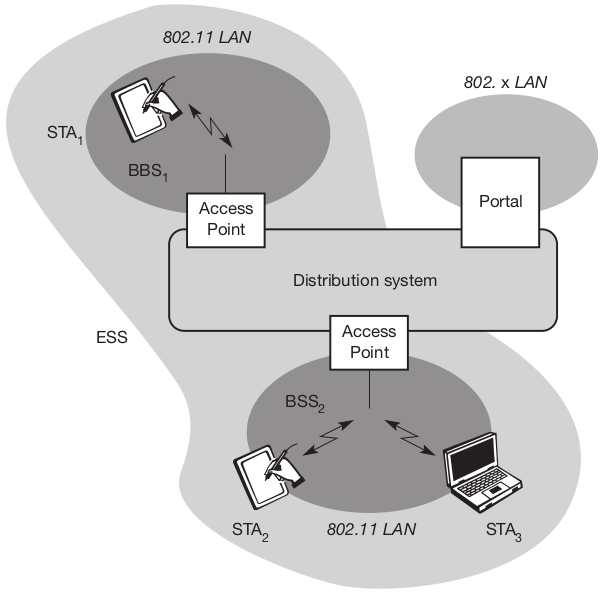
\includegraphics[width=0.7\textwidth]{architecture-of-ieee-802-11}
	\caption{Architecture of an infrastructure-based IEEE 802.11}\label{fig:architecture-of-ieee-802-11}
\end{figure}


\subsubsection[AP]{Access Point (AP)}
Several nodes, called \textbf{stations} ($STA_{i}$), are connected to \textbf{access points (AP)}.

\subsubsection[STA]{Stations (STA)}
 \textbf{Stations} are terminals with access mechanisms to the wireless medium and radio contact to the AP. 

\subsubsection[BSS]{Basic Service Set (BSS)}
The stations and the AP which are within the same radio coverage form a \textbf{basic service set} ($BSS_{i}$). The example shows two BSSs --- $ BSS_1 $ and $ BSS_2 $ --- which are connected via a distribution system. 

\subsubsection[ESS]{Extended Service Set (ESS)}
A distribution system connects several BSSs via the AP to form a single network and thereby extends the wireless coverage area. This network is now called an \textbf{extended service set (ESS)} and has its own identifier, the ESSID. The ESSID is the `name' of a network and is used to separate different networks. Without knowing the ESSID (and assuming no hacking) it should not be possible to participate in the WLAN. 

\subsubsection[Portal]{Portal}
The distribution system connects the wireless networks via the APs with a portal, which forms the interworking unit to other LANs.


\noindent The architecture of the distribution system is not specified further in IEEE 802.11. It could consist of bridged IEEE LANs, wireless links, or any other networks. However, \textbf{distribution system} services are defined in the standard

\subsubsection{Distribution System}
Stations can select an AP and associate with it. The APs support roaming (i.\ e.\ , changing access points), the distribution system handles data transfer between the different APs. 
\begin{itemize}
	\item APs provide synchronization within a BSS, 
	\item support power management, and 
	\item can control medium access to support time-bounded service. 
\end{itemize}


\noindent In addition to infrastructure-based networks, IEEE 802.11 allows the building of ad-hoc networks between stations, thus forming one or more independent BSSs (IBSS) as shown in Figure {\ref{fig:ad-hoc-wlan-architecture}}. In this case, an IBSS comprises a group of stations using the same radio frequency. Stations $STA_1$, $ STA_2 $, and $ STA_3 $ are in $ IBSS_1 $, $ STA_4 $ and $ STA_5 $ in $ IBSS_2 $. This means for example that $ STA_3 $ can communicate directly with $ STA_2 $ but not with $ STA_5 $. Several IBSSs can either be formed via the distance between the IBSSs (see Figure {\ref{fig:ad-hoc-wlan-architecture}}) or by using different carrier frequencies (then the IBSSs could overlap physically). 

%%%%%%%%%%%%%%%%%%%%%%%%%%%%%%%%%%%%%%%%%%%%%%
%				
%				Figure
%
%%%%%%%%%%%%%%%%%%%%%%%%%%%%%%%%%%%%%%%%%%%%%%
\begin{figure}[phb!]
	\centering
	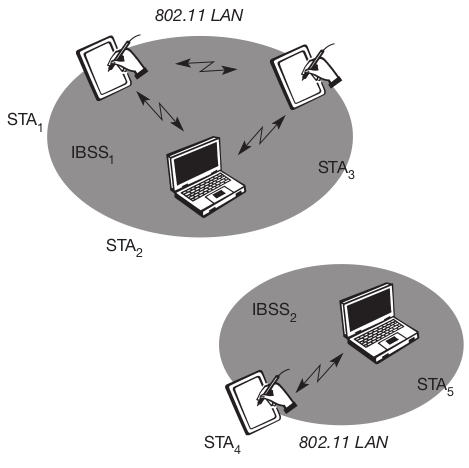
\includegraphics[width=0.7\textwidth]{ad-hoc-wlan-architecture}
	\caption{Architecture of IEEE 802.11 ad-hoc wireless LANs}\label{fig:ad-hoc-wlan-architecture}
\end{figure}

\subsection{Protocol Architecture}
IEEE 802.11 fits seamlessly into the other 802.x standards for wired LANs. Figure \ref{fig:ieee-802-11-protocol-architecture} shows the most common scenario: 
%\begin{multicols}{2}
	\begin{enumerate}
		\item An IEEE 802.11 wireless LAN connected to a switched IEEE 802.3 Ethernet via a bridge. 
		\item Applications should not notice any difference apart from the lower bandwidth and perhaps higher access time from the wireless LAN. 
		\item The WLAN behaves like a slow wired LAN. 
		\item Consequently, the higher layers (application, TCP, IP) look the same for wireless nodes as for wired nodes. 
		\item The upper part of the data link control layer, the logical link control (LLC), covers the differences of the medium access control layers needed for the different media.  
	\end{enumerate}
%\end{multicols}

%%%%%%%%%%%%%%%%%%%%%%%%%%%%%%%%%%%%%%%%%%%%%%
%				
%				Figure
%
%%%%%%%%%%%%%%%%%%%%%%%%%%%%%%%%%%%%%%%%%%%%%%
\begin{figure}[pht]
	\centering
	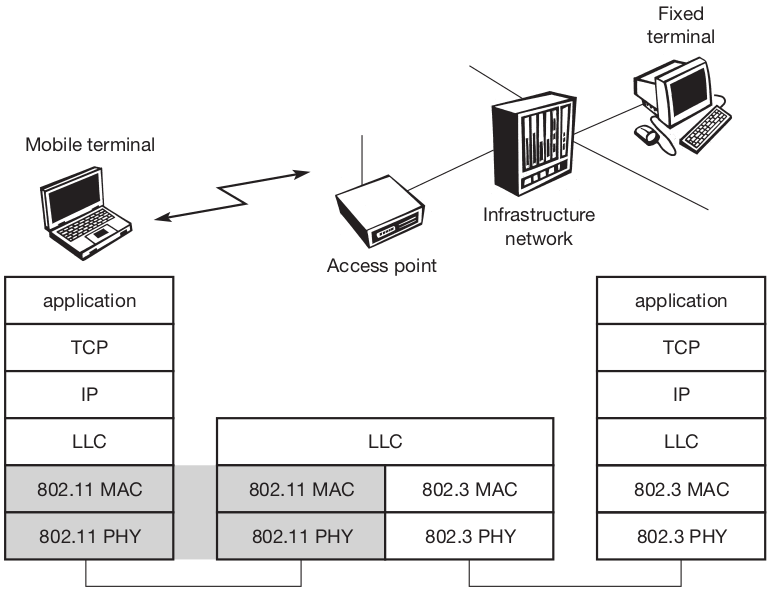
\includegraphics[width=0.8\textwidth]{ieee-802-11-protocol-architecture}
	\caption{IEEE 802.11 protocol architecture and bridging}\label{fig:ieee-802-11-protocol-architecture}
\end{figure}

In many of today’s networks, no explicit LLC layer is visible.



The IEEE 802.11 standard only covers the physical layer \textbf{PHY} and medium access layer \textbf{MAC} like the other 802.x LANs do.
%%%%%%%%%%%%%%%%%%%%%%%%%%%%%%%%%%%%%%%%%%%%%%
%				
%				Figure
%
%%%%%%%%%%%%%%%%%%%%%%%%%%%%%%%%%%%%%%%%%%%%%%

\begin{figure}[h!]
	\centering
	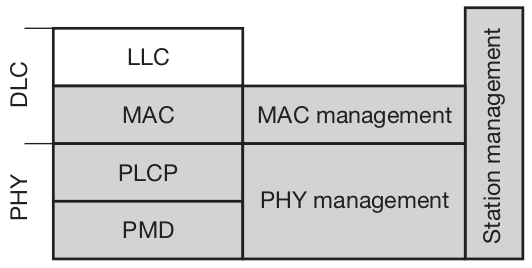
\includegraphics[width=0.8\textwidth]{ieee-802-11-protocol-architecture-and-management}
	\caption{Detailed IEEE 802.11 protocol architecture and management}\label{fig:ieee-802-11-protocol-architecture-and-management}
\end{figure}

\subsubsection[PHY]{Physical Layer}
 The physical layer is subdivided into:
 \begin{enumerate}
 	\item \textbf{physical layer convergence protocol (PLCP)} and 
 	\item \textbf{physical medium dependent} (\textbf{PMD}) sublayer (see Figure \ref{fig:ieee-802-11-protocol-architecture-and-management}). 
 \end{enumerate}


\paragraph{PLCP}
\begin{itemize}
	\item The PLCP sublayer provides a carrier sense signal, called clear \textit{channel assessment (CCA)}, and 
	\item provides a common PHY service access point (SAP) independent of the transmission technology. 
	\item Finally, the PMD sublayer handles modulation and encoding/decoding of signals. 
\end{itemize}


\subsubsection[MAC]{MAC Layer}
The basic tasks of the MAC layer comprise:
\begin{itemize}
	\item medium access, 
	\item fragmentation of user data, and 
	\item encryption.
\end{itemize}


\noindent Apart from the protocol sublayers, the standard specifies \textbf{management layers} and the \textbf{station management}. 

\subsubsection*{MAC Management}
\begin{itemize}
	\item The MAC management supports the association and re-association of a station to an access point and roaming between different access points. 
	\item It also controls authentication mechanisms, encryption, synchronization of a station with regard to an access point, and power management to save battery power. 
	\item MAC management also maintains the MAC	management information base (MIB).
\end{itemize}



\subsubsection*{PHY Management}
The main tasks of the PHY management include channel tuning and PHY MIB maintenance. 

\subsubsection*{Station Management}
Station management interacts with both management layers and is responsible for additional higher layer functions (e.\ g.\ , control of bridging and interaction with the distribution system in the case of an access point).



\subsection{802.11b}\label{sec:802.11b}

Soon after the first commercial 802.11 products came on the market some companies offered proprietary solutions. To avoid market
segmentation, a common standard, \textbf{IEEE 802.11b}\footnote{Do not
	get confused about the fact that 802.11b hit the market before 802.11a. The
	standards are named according to the order in which the respective study
	groups have been established.} soon followed and was added as supplement to the original standard (Higher-speed physical layer extension in the 2.4 GHz band). 


\begin{itemize}
	\item This standard describes a new PHY layer.
	\item Depending on the interference and the distance between sender and receiver 802.11b systems offer $ 11 $, $ 5.5 $, $ 2 $, or $ 1 Mbit/s $. 
	\item Maximum user data rate is approx $ 6 Mbit/s $.
	\item The standard defines several packet formats for the physical layer.
	\item The mandatory format interoperates with the original versions of 802.11. 
	\item The optional versions provide a more efficient data transfer due to shorter headers/different coding schemes and can coexist with other 802.11 versions.
	\item The standards operates on certain frequencies in the 2.4 GHz ISM band. These depend on national regulations.
	\item Devices using 802.11b experience interference from other products operating in the 2.4 GHz band.
	\item \textbf{Pros of 802.11b}: lowest cost; signal range is good and not easily obstructed.
	\item \textbf{Cons of 802.11b}: slowest maximum speed; home appliances may interfere on the unregulated frequency band.
\end{itemize}


\subsection{802.11a} \label{sec:802.11a}
While 802.11b was in development, IEEE created a second extension to the original 802.11 standard called 802.11a. Because 802.11b gained in popularity much faster than did 802.11a.

\begin{itemize}
	\item Uses the same data link layer protocol and frame format as the original standard, but an OFDM\footnote{orthogonal frequency-division multiplexing (OFDM) is a type of digital transmission and a method of encoding digital data on multiple carrier frequencies.} based air interface (physical layer).
	\item It operates in the 5 GHz band with a maximum net data rate of $ 54 Mbit/s $.
	\item The higher frequency also means 802.11a signals have more difficulty penetrating walls and other obstructions.
	\item Because 802.11a and 802.11b utilize different frequencies, the two technologies are incompatible with each other. 
	\item \textbf{Pros of 802.11a}: fast maximum speed; regulated frequencies prevent signal interference from other devices.
	\item \textbf{Cons of 802.11a}: highest cost; shorter range signal that is more easily obstructed.
\end{itemize}


\subsection{Newer Developments} \label{sec:newer-developments}
While many products that follow the IEEE 802.11a and 802.11b standards are available, several new groups have been formed within the IEEE to discuss enhancements of the standard and new applications.

\begin{itemize}
\item \textbf{802.11e (MAC enhancements)}: For applications such as audio, video, or media stream, distribution service classes have to be provided. For this
reason, the MAC layer must be enhanced compared to the current standard.

\item \textbf{802.11f (Inter-Access Point Protocol)}: The standard currently only describes the basic architecture of 802.11 networks and their components. 

\item \textbf{802.11g (Data rates above 20 Mbit/s at 2.4 GHz)}: Introducing new modulation schemes, forward error correction and OFDM also allows for higher data
rates at 2.4 GHz. This approach should be backward compatible to 802.11b
and should benefit from the better propagation characteristics at 2.4 GHz compared to 5 GHz.

\item \textbf{802.11h (Spectrum managed 802.11a)}: The 802.11a standard was primarily designed for usage in the US U-NII bands. The standardization did not consider non-US regulations such as the European requirements for power control and dynamic selection of the transmit frequency. To enable the regulatory acceptance of 5 GHz products, dynamic channel selection (DCS) and transmit power control (TPC) mechanisms (as also specified for the European HiperLAN2 standard) have been added. With this extension, 802.11a products can also be operated in Europe. These additional mechanisms try to balance the load in the 5 GHz band.

\item \textbf{802.11i (Enhanced Security mechanisms)}: As the original security mechanisms (WEP) proved to be too weak soon after the deployment of the first products, this working group discusses stronger encryption and authentication mechanisms. IEEE 802.1x will play a major ⎄role in this process.
\end{itemize}

\subsection{HIPERLAN 1} \label{sec:hiperlan-1}
In 1996, the ETSI standardized HIPERLAN 1 as a WLAN allowing for node mobility and supporting ad-hoc and infrastructure-based topologies. (HIPERLAN stands for \textbf{high performance local area network}.) \textbf{HIPERLAN 1} was originally one out of four HIPERLANs envisaged, as ETSI decided to have different types of networks for different purposes. The key feature of all
four networks is their integration of time-sensitive data transfer services. Over time, names have changed and the former HIPERLANs 2, 3, and 4 are now called HiperLAN2, HIPERACCESS, and HIPERLINK.

The service offered by a HIPERLAN 1 is compatible with the standard MAC services known from IEEE 802.x LANs

An innovative feature of HIPERLAN 1, which many other wireless networks do not offer, is its ability to forward data packets using several relays. Relays can extend the communication on the MAC layer beyond the radio range.

HiperLAN features:

\begin{itemize}
	\item range $ 100 m $
\item slow mobility ($ 1.4 m/s $)
\item supports asynchronous and synchronous traffic
\item Bit rate - $ 23.59 Mbit/s $
\end{itemize}


\subsection{HIPERLAN 2} \label{sec:hiperlan-2}
While HIPERLAN 1 did not succeed HiperLAN2 might have a better chance. (This is also written as HIPERLAN/2, HiperLAN/2, H/2) Standardized by ETSI this wireless network works at 5 GHz  and offers data rates of up to $ 54 Mbit/s $ including QoS support and enhanced security features. In comparison with basic IEEE 802.11 LANs, HiperLAN2 offers more features in the mandatory parts
of the standard.

Features:

\subsubsection*{High-throughput transmission}
\begin{itemize}
	\item HiperLAN2 not only offers up to $ 54 Mbit/s $ at the physical layer but also about $ 35 Mbit/s $ at the network layer.
	\item The overheads introduced by the layers (medium access, packet headers etc.) remain almost constant over a wide range of user packet sizes and Data rates.
\end{itemize}

\subsubsection*{Connection-oriented}
Prior to data transmission HiperLAN2 networks establish logical connections between a sender and a receiver.


\subsubsection*{Quality of service support}
With the help of connections, support of QoS is much simpler. Each connection has its own set of QoS parameters.

\subsubsection*{Dynamic frequency selection}
\begin{itemize}
	\item HiperLAN2 does not require frequency planning.
	\item All access points have built-in support which automatically selects an appropriate frequency within their coverage area.
\end{itemize}

\subsubsection*{Security support}
Authentication as well as encryption is supported by HiperLAN2.

\subsubsection*{Mobility support}
\begin{itemize}
	\item Mobile terminals can move around while transmission always takes place between the terminal and the access point with the best radio signal.
	\item Handover between access points is performed automatically.
\end{itemize}

\section{Bluetooth} \label{sec:bluetooth}
Compared to the WLAN technologies, the Bluetooth technology aims at so-called \textbf{ad-hoc piconets}, which are local area networks with a very limited coverage and without the need for an infrastructure. This is a different type of network is needed to connect different
small devices in close proximity (about 10 m) without expensive wiring or the need for a wireless infrastructure. 

Swedish IT-company Ericsson initiated some studies in 1994 around a so-called multi-communicator link. The project was renamed and Bluetooth was born. In spring 1998 five companies (Ericsson, Intel, IBM, Nokia, Toshiba) founded the Bluetooth consortium with the goal of developing a single-chip, low-cost, radio-based wireless network technology. Many other companies and research institutions joined the special interest group around Bluetooth, whose goal was the development of mobile phones, laptops, notebooks, headsets etc. including Bluetooth technology, by the end of 1999. 

In 2001, the first products hit the mass market, and many mobile phones, laptops, PDAs, video cameras etc. are equipped with Bluetooth technology today.


\subsection{User Scenarios}
Many different user scenarios can be imagined for wireless piconets or WPANs:

\begin{itemize}
\item \textbf{Connection of peripheral devices}: Today, most devices are connected to a desktop computer via wires (e.\ g.\ , keyboard, mouse, joystick, headset, speakers). This type of connection has several disadvantages: each device has its
own type of cable, different plugs are needed, wires block office space. In a
wireless network, no wires are needed for data transmission. However, batteries now have to replace the power supply, as the wires not only transfer
data but also supply the peripheral devices with power.

\item \textbf{Support of ad-hoc networking}: Imagine several people coming together,
discussing issues, exchanging data (schedules, sales figures etc.). For
instance, students might join a lecture, with the teacher distributing data to
their personal digital assistants (PDAs). Wireless networks can support this
type of interaction; small devices might not have WLAN adapters following
the IEEE 802.11 standard, but cheaper Bluetooth chips built in.

\item \textbf{Bridging of networks}: Using wireless piconets, a mobile phone can be connected to a PDA or laptop in a simple way. Mobile phones have a Bluetooth chip. The mobile phone
can then act as a bridge between the local piconet and, e.\ g.\ , the global GSM
network. 
\end{itemize}

When comparing Bluetooth with other WLAN technology we have to keep
in mind that one of its goals was to provide local wireless access at very low
cost. From a technical point of view, WLAN technologies like those above could
also be used, however, WLAN adapters, e.\ g.\ , for IEEE 802.11, have been
designed for higher bandwidth and larger range and are more expensive and
consume a lot more power.

\subsection{Architecture} \label{sec:bluetooth-architecture}
Like IEEE 802.11b, Bluetooth operates in the 2.4 GHz ISM band. However, MAC, physical layer and the offered services are completely different.

\subsubsection*{Networking}
Bluetooth operates on 79 channels in the 2.4 GHz band with 1 MHz carrier spacing. Each device performs frequency hopping with
1,600 hops/s in a pseudo random fashion. 

A very important term in the context of Bluetooth is a \textbf{piconet}. 

\subsubsection{Piconet}
A piconet is a collection of Bluetooth devices which are synchronized to the same hopping
sequence. Figure {\ref{fig:bluetooth-piconet}} shows a collection of devices with different roles.
\begin{enumerate}
	\item One device in the piconet can act as \textbf{master} (M) all other devices connected to the master must act as \textbf{slaves} (S)
	\item The master determines the hopping pattern in the piconet and the slaves have to synchronize to this pattern.
	\item Each piconet has a unique hopping pattern. If a device wants to participate it has to synchronize to
	this.
	\item Two additional types of devices are shown: 
	\begin{itemize}
		\item \textbf{parked devices} (P) can not actively participate in the piconet (e.\ g.\ , they do not have a connection), but are
		known and can be reactivated within some milliseconds.
		\item Devices in \textbf{stand-by} (SB) do not participate in the piconet.
	\end{itemize}
\end{enumerate}

\begin{multicols}{2}
	\begin{itemize}
		\item Each piconet has exactly one master and up to seven simultaneous slaves. 
		\item More than 200 devices can be parked. 
		\item The reason for the upper limit of eight active devices, is the 3-bit address used in Bluetooth. 
		\item If a parked device wants to communicate and there are already seven active slaves, one slave has to switch to park mode to allow the parked device to switch to active mode.
	\end{itemize}
\end{multicols}


%%%%%%%%%%%%%%%%%%%%%%%%%%%%%%%%%%%%%%%%%%%%%%
%				
%				Figure
%
%%%%%%%%%%%%%%%%%%%%%%%%%%%%%%%%%%%%%%%%%%%%%%

\begin{figure}[h!]
\centering
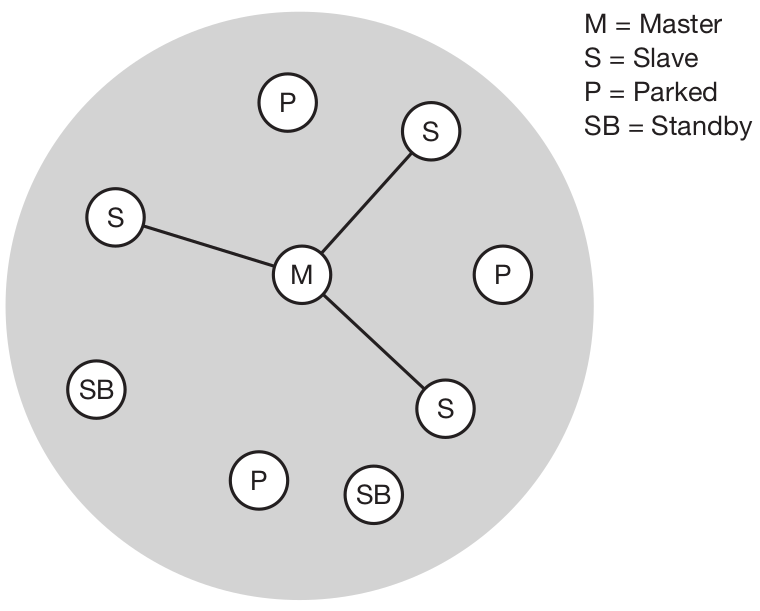
\includegraphics[width=0.8\textwidth]{bluetooth-piconet}
\caption{Simple Bluetooth piconet}\label{fig:bluetooth-piconet}
\end{figure}

\subsubsection{Scatternet}
All users within one piconet have the same hopping sequence and share the same 1 MHz channel. As more users join the piconet, the throughput per user drops quickly. This led to the idea of forming groups of piconets called \textbf{scatternet}. Only those units that really must exchange data share the same piconet, so that many piconets with overlapping coverage can exist simultaneously.


%%%%%%%%%%%%%%%%%%%%%%%%%%%%%%%%%%%%%%%%%%%%%%
%				
%				Figure
%
%%%%%%%%%%%%%%%%%%%%%%%%%%%%%%%%%%%%%%%%%%%%%%

\begin{figure}[h!]
\centering
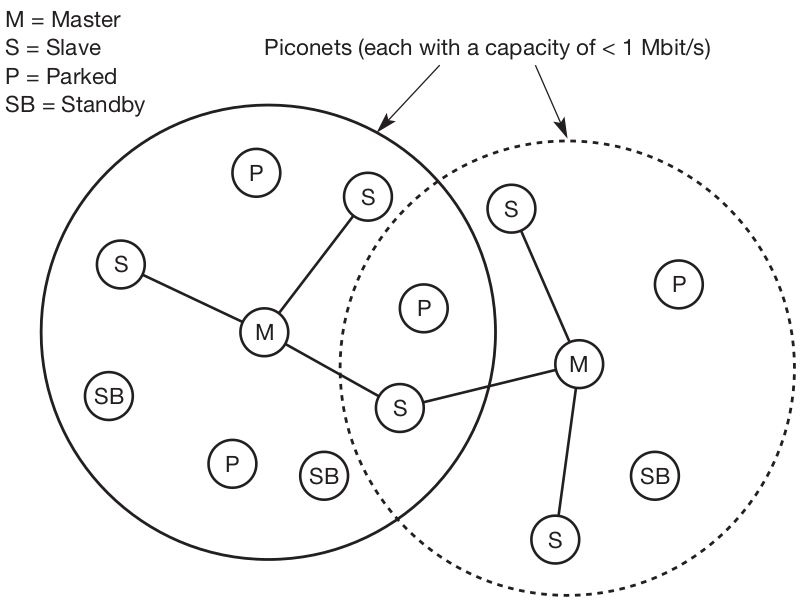
\includegraphics[width=0.8\textwidth]{bluetooth-scatternet}
\caption{Bluetooth scatternet}\label{fig:bluetooth-scatternet}
\end{figure}

In the example, 
\begin{multicols}{2}
	\begin{enumerate}
		\item the scatternet consists of two piconets, in which one device participates in two different piconets.
		\item Both piconets use a different hopping sequence, always determined by the master of the piconet. 
		\item In an average sense, all piconets can share the total of 80 MHz bandwidth available. 
		\item Adding more piconets leads to a graceful performance degradation of a single piconet because more and more
		collisions may occur. 
		\item A collision occurs if two or more piconets use the same carrier frequency at the same time. 
	\end{enumerate}
\end{multicols}



If a device wants to participate in more than one piconet:
\begin{multicols}{2}
\begin{itemize}
	\item It has to synchronize to the hopping sequence of the piconet it wants to take part in. 
	\item If a device acts as slave in one piconet, it simply starts to synchronize with the hopping sequence of the piconet it wants to join. 
	\item After synchronization, it acts as a slave in this piconet and no longer participates in its former piconet.
	\item Before leaving one piconet, a slave informs the current master that it will be unavailable for a certain amount of time. 
	\item The remaining devices in the piconet continue to communicate as usual.
\end{itemize}
\end{multicols}


A master can also leave its piconet and act as a slave in another piconet. As soon as a master leaves a piconet, all traffic within this piconet is suspended until the master returns.

Communication between different piconets takes place by devices jumping back and forth between theses nets. 

\subsection{Protocol Stack}
Bluetooth protocol stack can be thought of as a combination of multiple application specific stacks.

The Bluetooth protocol stack can be divided into a \textit{core specification}, which describes the protocols from physical layer to the data link control together with management functions, and \textbf{profile specifications}. The latter describes many protocols and functions needed to adapt the wireless Bluetooth technology to legacy and new applications.



%%%%%%%%%%%%%%%%%%%%%%%%%%%%%%%%%%%%%%%%%%%%%%
%				
%				Figure
%
%%%%%%%%%%%%%%%%%%%%%%%%%%%%%%%%%%%%%%%%%%%%%%

\begin{figure}[h]
\centering
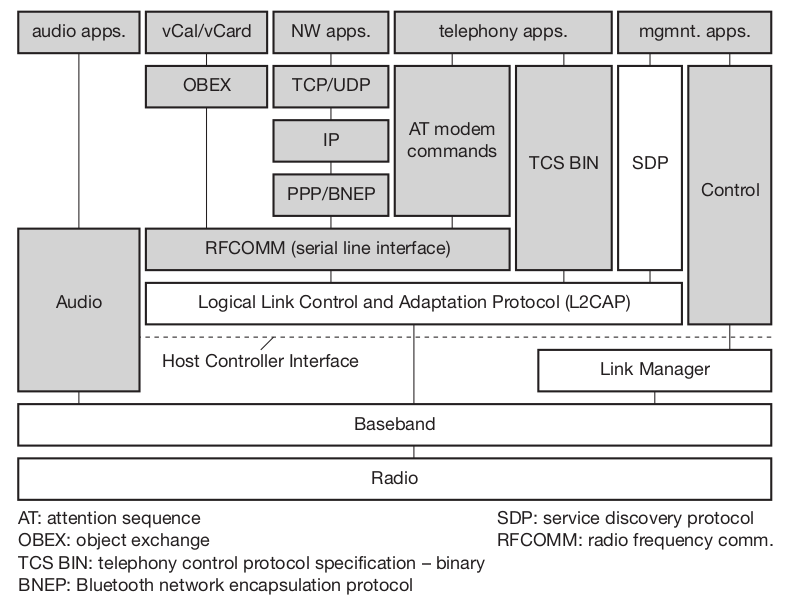
\includegraphics[width=0.8\textwidth]{bluetooth-protocol-stack}
\caption{Bluetooth protocol stack}\label{fig:bluetooth-protocol-stack}
\end{figure}

Bluetooth protocol stack (see figure \ref{fig:bluetooth-protocol-stack}) can be divided into different components according to their functions.

\subsubsection{Core Protocols}
The \textbf{core protocols} of Bluetooth comprise the following elements:
\begin{itemize}
\item \textbf{Radio}: Specification of the air interface, e.\ g.\ , frequencies, modulation, and transmit power.

\item \textbf{Baseband}: Description of basic connection establishment, packet formats, timing, and basic QoS parameters.

\item \textbf{Link manager protocol}: Link set-up and management between devices including security functions and parameter negotiation.

\item \textbf{Logical link control and adaptation protocol (L2CAP)}: Adaptation of higher layers to the baseband (connectionless and connection-oriented services).

\item \textbf{Service discovery protocol}: Device discovery in close proximity plus querying of service characteristics.
\end{itemize}

\subsubsection{Cable Replacement Protocol}
On top of L2CAP is the \textbf{cable replacement protocol} RFCOMM that emulates a serial line interface.
\begin{itemize}
	\item This allows for a simple replacement of serial line cables and enables many legacy applications and protocols to run over Bluetooth. 
	\item RFCOMM supports multiple serial ports over a single physical channel. 
	
\end{itemize}

\subsubsection{Telephony Control Protocol}
\begin{itemize}
	\item The \textbf{telephony control protocol specification - binary (TCS BIN)} describes a bit-oriented protocol that defines
	call control signaling for the establishment of voice and data calls between Bluetooth devices. 
	\item It also describes mobility and group management functions.
\end{itemize}

\subsubsection{Adopted Protocols}
Many protocols have been adopted in the Bluetooth standard. 
\begin{itemize}
	\item Classical Internet applications can still use the standard \textbf{TCP/IP} stack running over PPP or use the more efficient \textbf{Bluetooth network encapsulation protocol (BNEP)}. 
	\item Telephony applications can use the \textbf{AT modem commands} as if they were using a standard modem. 
	\item \textbf{Calendar and business card objects (vCalendar/vCard}) can be exchanged using the \textbf{object exchange protocol (OBEX)} as common with IrDA interfaces.
\end{itemize}



\subsubsection[Host Controller Interface]{Host Controller Interface (HCI)}
\begin{itemize}
	\item The HCI between the baseband and L2CAP provides a command interface to the baseband controller and link manager, and access to the hardware status and control registers. 
	\item The HCI can be seen as the hardware/software boundary.
\end{itemize}

\subsubsection{Audio}
\begin{itemize}
	\item A real difference to other protocol stacks is the support of audio. 
	\item Audio applications may directly use the baseband layer after encoding the audio signals.
\end{itemize}

	\begin{center}
\begin{framed}
	\begin{nepali}
		ब्लुटुथ प्राेटाेकल स्ट्याककाे सरल चित्र। माथि चित्रण गरिएकाे चित्रकाे साटाे याे बनाएपनि हुन्छ। (Simplified figure of Bluetooth protocol stack.)
	\end{nepali}
\end{framed}
\end{center}
\begin{figure*}[bph]
	\centering
	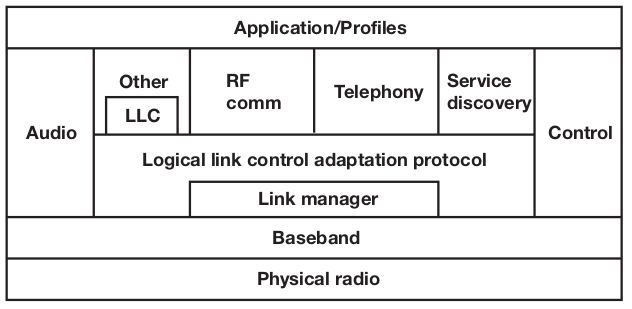
\includegraphics[width=0.7\textwidth]{bluetooth-protocol-stack-alternative}
%	\caption{Bluetooth protocol stack}
	\label{fig:bluetooth-protocol-stack-alternative}
\end{figure*}

\begin{figure}

\end{figure}

